\documentclass{article}

\usepackage{amsmath,amssymb}
\usepackage{tikz}
\usepackage{pgfplots}
\usepackage{xcolor}
\usepackage[left=2.1cm,right=3.1cm,bottom=3cm,footskip=0.75cm,headsep=0.5cm]{geometry}
\usepackage{enumerate}
\usepackage{enumitem}
\usepackage{marvosym}
\usepackage{tabularx}
\usepackage{multirow}

\usepackage[utf8]{inputenc}

\renewcommand*{\arraystretch}{1.4}

\newcolumntype{L}[1]{>{\raggedright\arraybackslash}p{#1}}
\newcolumntype{R}[1]{>{\raggedleft\arraybackslash}p{#1}}
\newcolumntype{C}[1]{>{\centering\let\newline\\\arraybackslash\hspace{0pt}}m{#1}}

\title{\textbf{Rechtfertigung der Staatstätigkeit, Hausaufgabe 3}}
\author{\textsc{Henry Haustein}}
\date{}

\begin{document}
	\maketitle
	
	\section*{Aufgabe 1}
	\begin{enumerate}[label=(\alph*)]
		\item Die Straße würde 20 Mio. Euro kosten, aber einen Nutzen von $2\cdot 14$ Mio. Euro bringen. Aus gesamtwirtschaftlicher Sicht lohnt es sich also die Straße zu bauen.
		\item Auszahlungsmatrix, der Zeilenspieler wird zuerst genannt:
		\begin{center}
			\begin{tabular}{C{0.5cm}c|c|c}
				& & \multicolumn{2}{c}{\textbf{Bedorf}} \\
				& & bauen & nicht bauen \\
				\hline
				\multirow{2}{0.5cm}{\rotatebox[origin=c]{90}{\textbf{Adorf}}} & bauen & (4,4) & (-6,14) \\
				\cline{3-4}
				& nicht bauen & (14,-6) & (0,0)
			\end{tabular}
		\end{center}
		\textit{nicht bauen} ist also eine dominante Strategie, das Nash-Gleichgewicht ist daher (nicht bauen, nicht bauen).
		\item Auszahlungsmatrix, der Zeilenspieler wird zuerst genannt:
		\begin{center}
			\begin{tabular}{C{0.5cm}c|c|c}
				& & \multicolumn{2}{c}{\textbf{Bedorf}} \\
				& & bauen & nicht bauen \\
				\hline
				\multirow{2}{0.5cm}{\rotatebox[origin=c]{90}{\textbf{Adorf}}} & bauen & (20,1) & (10,11) \\
				\cline{3-4}
				& nicht bauen & (30,-9) & (0,0)
			\end{tabular}
		\end{center}
		Falls Bedorf baut, baut Adorf nicht und falls Bedorf nicht baut, baut Adorf. \\
		Falls Adorf baut, baut Bedorf nicht und falls Adorf nicht baut, baut Bedorf nicht. \\
		Für Bedorf ist \textit{nicht bauen} eine dominante Strategie; das Nash-Gleichgewicht ist (bauen, nicht bauen)
	\end{enumerate}
	
	\section*{Aufgabe 3}
	\begin{enumerate}[label=(\alph*)]
		\item Die Grenzkosten betragen 30. Unter Wohlfahrtsgesichtspunkten liefert $\sum GZB = GK$ die optimale Lösung, also
		\begin{align}
			\sum GZB &= GK \notag \\
			(40-2G) + (20-G) &= 30 \notag \\
			60-3G &= 30 \notag \\
			G_{opt} &= 10 \notag
		\end{align}
		\item Für Haushalt 1 gilt:
		\begin{align}
			GZB_1 &= \alpha \cdot GK \notag \\
			40-2G &= \frac{1}{2} \cdot 30 \notag \\
			G_1 &= 12.5 \notag
		\end{align}
		Für Haushalt 2 gilt:
		\begin{align}
			GZB_2 &= (1-\alpha) \cdot GK \notag \\
			20-G &= \left(1-\frac{1}{2}\right) \cdot 30 \notag \\
			G_2 &= 5 \notag
		\end{align}
		Die Haushalte fragen verschiedene Mengen nach, aber es kann nur eine Menge bereitgestellt werden.
		\begin{center}
			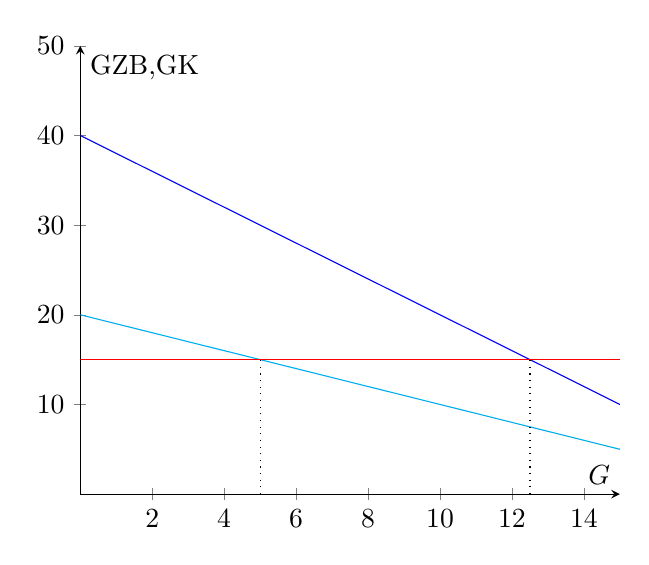
\begin{tikzpicture}
				\begin{axis}[
					xmin=0, xmax=15, xlabel=$G$,
					ymin=0, ymax=50, ylabel={GZB,GK},
					samples=400,
					axis x line=middle,
					axis y line=middle,
					domain=0:15
					]
					\addplot[mark=none,smooth,blue] {40-2*x};
					\addplot[mark=none,smooth,cyan] {20-x};
					
					\addplot[mark=none,smooth,red] {15};
					
					\draw[dotted] (axis cs: 5,0) -- (axis cs: 5,15);
					\draw[dotted] (axis cs: 12.5,0) -- (axis cs: 12.5,15);
					
				\end{axis}
			\end{tikzpicture} \\
			\textcolor{red}{$\alpha GK = (1-\alpha)GK$}, \textcolor{blue}{$GZB_1$}, \textcolor{cyan}{$GZB_2$}
		\end{center}
		\item Wir müssen $\alpha^\ast$ so wählen, dass
		\begin{align}
			GZB_1(G_{opt}) &= \alpha^\ast \cdot GK \notag \\
			40-2\cdot 10 &= \alpha^\ast \cdot 30 \notag \\
			20 &= \alpha^\ast \cdot 30 \notag \\
			\alpha^\ast &= \frac{2}{3} \notag
		\end{align}
		Der andere Haushalt muss dann $1-\alpha$ der Grenzkosten tragen, für ihn sind das $\frac{1}{3}$ der Grenzkosten.
		\begin{center}
			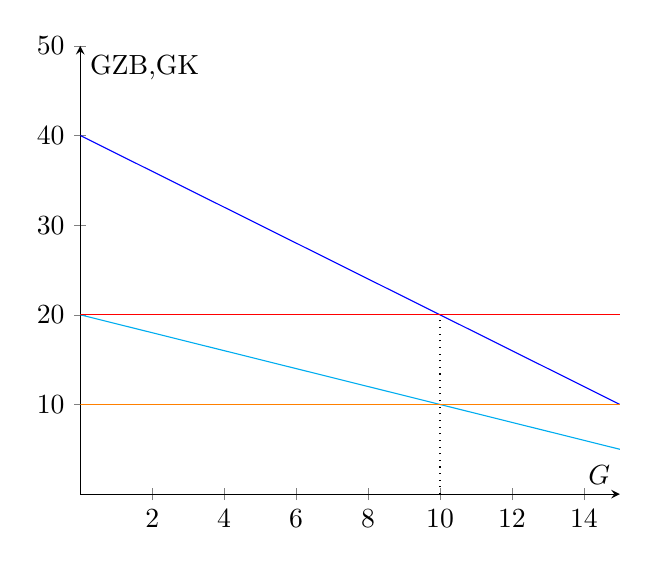
\begin{tikzpicture}
				\begin{axis}[
					xmin=0, xmax=15, xlabel=$G$,
					ymin=0, ymax=50, ylabel={GZB,GK},
					samples=400,
					axis x line=middle,
					axis y line=middle,
					domain=0:15
					]
					\addplot[mark=none,smooth,blue] {40-2*x};
					\addplot[mark=none,smooth,cyan] {20-x};
					
					\addplot[mark=none,smooth,red] {20};
					\addplot[mark=none,smooth,orange] {10};
					
					\draw[dotted] (axis cs: 10,0) -- (axis cs: 10,20);
					
				\end{axis}
			\end{tikzpicture} \\
			\textcolor{blue}{$GZB_1$}, \textcolor{cyan}{$GZB_2$}, \textcolor{red}{$\alpha\cdot GK$}, \textcolor{orange}{$(1-\alpha)\cdot GK$}
		\end{center}
	\end{enumerate}

\end{document}